%\documentclass[10pt]{witseiepaper}
\documentclass[10pt, onecolumn]{IEEEtran}
\usepackage{tikz}
\usetikzlibrary{shapes, arrows}
%\usepackage{KJN}
\usepackage[colorlinks = true,
            linkcolor = black,
            urlcolor  = blue,
            citecolor = blue,
            anchorcolor = blue]{hyperref}
\usepackage[utf8]{inputenc}
\usepackage{circuitikz}
\usepackage{tikz}
\usepackage{amsmath,amsfonts,amssymb}
\usepackage{algorithmic}
\usepackage{pgfplots}
\usepackage{pgfgantt}
\usepackage{algorithm}
\usepackage{array}
\usepackage[caption=false,font=normalsize,labelfont=sf,textfont=sf]{subfig}
\usepackage{textcomp}
\usepackage{stfloats}
\usepackage{url}
\usepackage{verbatim}
\usepackage{graphicx}
\usepackage[T1]{fontenc}
\usepackage{lmodern}

\usepackage{graphicx}
\usepackage{color}
\usepackage{epstopdf}
\usepackage{subfig}
\usepackage{float}
\graphicspath{ {figures/} }
\usepackage{array}
\usepackage{multicol}
\pagestyle{plain}
\usepackage{pdfpages}
\usepackage{svg}
\usepackage{fancyvrb,newverbs,xcolor}
\definecolor{cverbbg}{gray}{0.93}
\newenvironment{lcverbatim}
 {\SaveVerbatim{cverb}}
 {\endSaveVerbatim
  \flushleft\fboxrule=0pt\fboxsep=.5em
  \colorbox{cverbbg}{%
    \makebox[\dimexpr\linewidth-2\fboxsep][l]{\BUseVerbatim{cverb}}%
  }
  \endflushleft
}
\usepackage{fancyhdr}
\usepackage{lastpage}
\usepackage{refcount}
\usepackage{ifthen}
\usepackage[sort&compress, numbers]{natbib}
\usepackage[none]{hyphenat}

\usepackage[subtle]{savetrees}
\begin{document}

\pagenumbering{arabic}
\pagestyle{fancy}
\renewcommand{\headrulewidth}{0pt}
\renewcommand{\footrulewidth}{0pt}
\fancyhead[L]{WITs HPC SIG}
\fancyhead[R]{ISC25 - Proposal for Participation}
\fancyfoot[C]{Page \thepage\ of \pageref{lastBodyPage}}
\begin{center}
    \LARGE{\textbf{University of the Witwatersrand, High Performance Computing Special Interest Group - Proposal for Participation}}
    \\
    %\large{Group, Date:~\\Authors}
\end{center}
\vspace{0.3cm}
  
\renewenvironment{abstract}
 {\par\noindent\textbf{\abstractname:}\ \ignorespaces}
 {\par\medskip}
%\begin{abstract}
%Abstract
%\end{abstract}
%\providecommand{\keywords}[1]
%{
% \textbf{Keywords: } #1
%}
%\noindent
%\keywords{Keywords}
%\begin{multicols*}{2}
\section{Introduction to our group}
\noindent
\IEEEPARStart{T}{he} \textbf{University of the Witwatersrand (Wits)}, located in Johannesburg, South Africa, is home to the \textbf{Wits HPC Special Interest Group (SIG)}, an active student-led organization dedicated to fostering knowledge and practical skills in high-performance computing among undergraduates. Our group’s primary objective is to educate students on HPC and prepare them for participation in the Centre for High Performance Computing (CHPC) Student Cluster Competition (SCC). 
\\\\
Our work has been highlighted through a \href{https://dl.acm.org/doi/10.1145/3626203.3670573}{published poster} that showcases how we utilize decommissioned hardware to train teams. Additionally, we will be presenting a paper at SC25 that delves into the operational framework of our group under the session \href{https://sc24.conference-program.com/session/?sess=sess752#:~:text=From%20Student%20SIG,PooleDavid%20Macleod} {"Best Practices for HPC Training and Education"}. Notably, a significant portion of Team CHPC at the International Supercomputing Conference (ISC) Student Cluster Competition (SCC) has historically been comprised of Wits students \href{https://witshpc.com}{historically comprised of Wits students}. 
\\\\
To broaden our scope and foster international collaboration, we aim to participate as an independent organization in this year’s ISC SCC. Our goal is to establish a sustainable pipeline that enables the group to field its own team for international competitions annually, ensuring consistent growth and global engagement for future members.
\section{Educational Institution Information}
\noindent
The University of the Witwatersrand, commonly known as Wits University (pronounced "V-its"), is a leading institution of higher learning based in Johannesburg, South Africa.

\vspace{0.05\textwidth}
\noindent
\begin{minipage}{0.45\textwidth}
  \centering
  
\includegraphics[width=0.6\textwidth]{wits_logo.png}
  \textbf{Wits University Logo} 
\end{minipage}
\hspace{0.05\textwidth} % Space between the images
\begin{minipage}{0.45\textwidth}
  \centering
  
\includegraphics[width=0.65\textwidth]{witshpc_logo_transparentbkg.png}
  \textbf{Wits HPC Special Interest Group} 
\end{minipage}
\\\\
\section{Team Captain Information}
\noindent
\begin{minipage}{0.2\textwidth}
  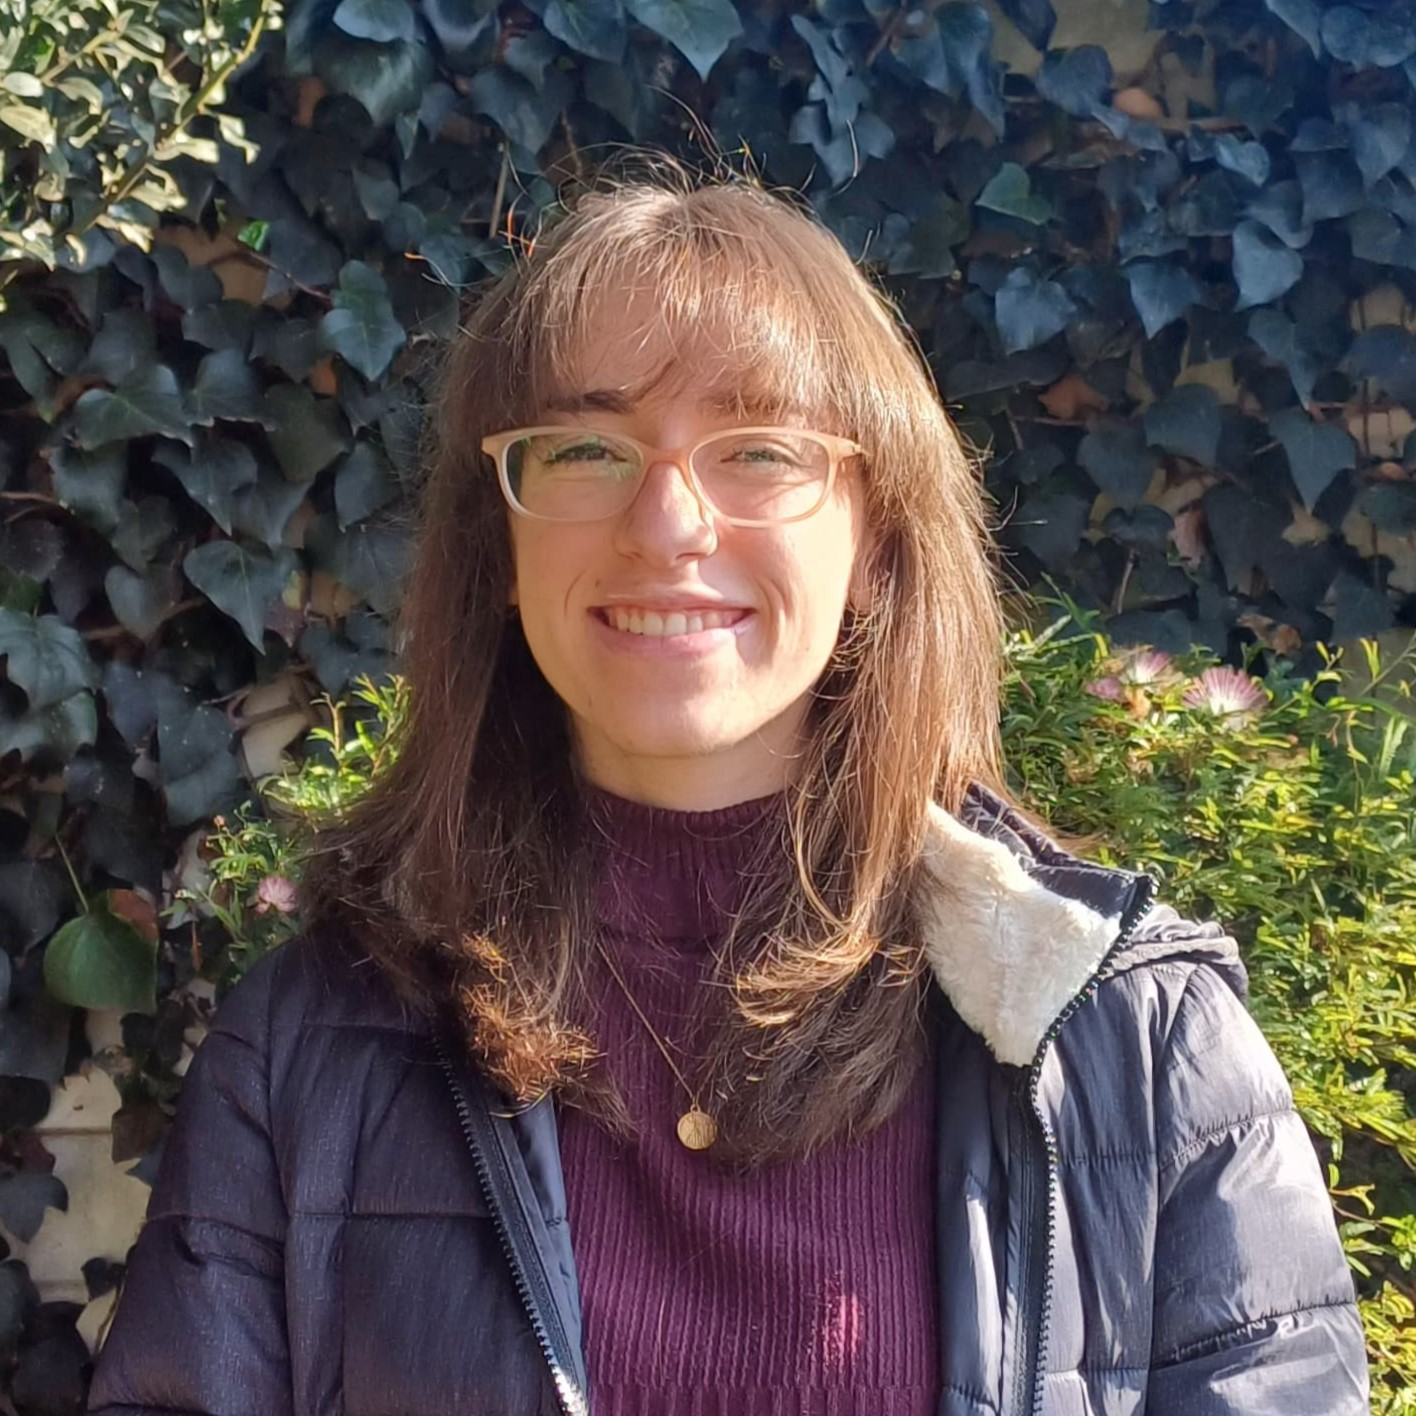
\includegraphics[width=\textwidth]{lily_photo.jpg}
\end{minipage}
\hspace{0.02\textwidth} % Space between image and text
\begin{minipage}{0.65\textwidth}
  \textbf{Lily de Melo} is an organiser with the Wits HPC Special Interest Group, where she helps coordinate group activities. She is currently in her second year of studying for a Bachelor's degree in Computer Science. Lily has gained substantial experience in high-performance computing through her active participation in the Wits SIG and previous SCCs. Notably, she was part of the winning team at the CHPC SCC 2023 and represented Team CHPC at ISC SCC 2024. Her motivation is to expand HPC education and opportunities for undergraduates at Wits, fostering a robust learning environment for future HPC enthusiasts.
\end{minipage}
\\\\

\noindent
\begin{minipage}{0.45\textwidth}
  \raggedright
  \textbf{Full Name:} Lily Sarah de Melo \\
  \textbf{Email:} lily.demelo@outlook.com \\
  \textbf{Cell:} +27 76 020 7973 \\
\end{minipage}
\hfill
\begin{minipage}{0.45\textwidth}
  \raggedright
  \textbf{Address:} \\
  14 Tarentaal Avenue \\
  Bassonia \\
  Johannesburg \\ 
  2190 \\
  South Africa \\
\end{minipage}
\\\\

\section{Team Member Information}
\vspace{0.02\textwidth} 
\noindent
\begin{minipage}{0.2\textwidth}
  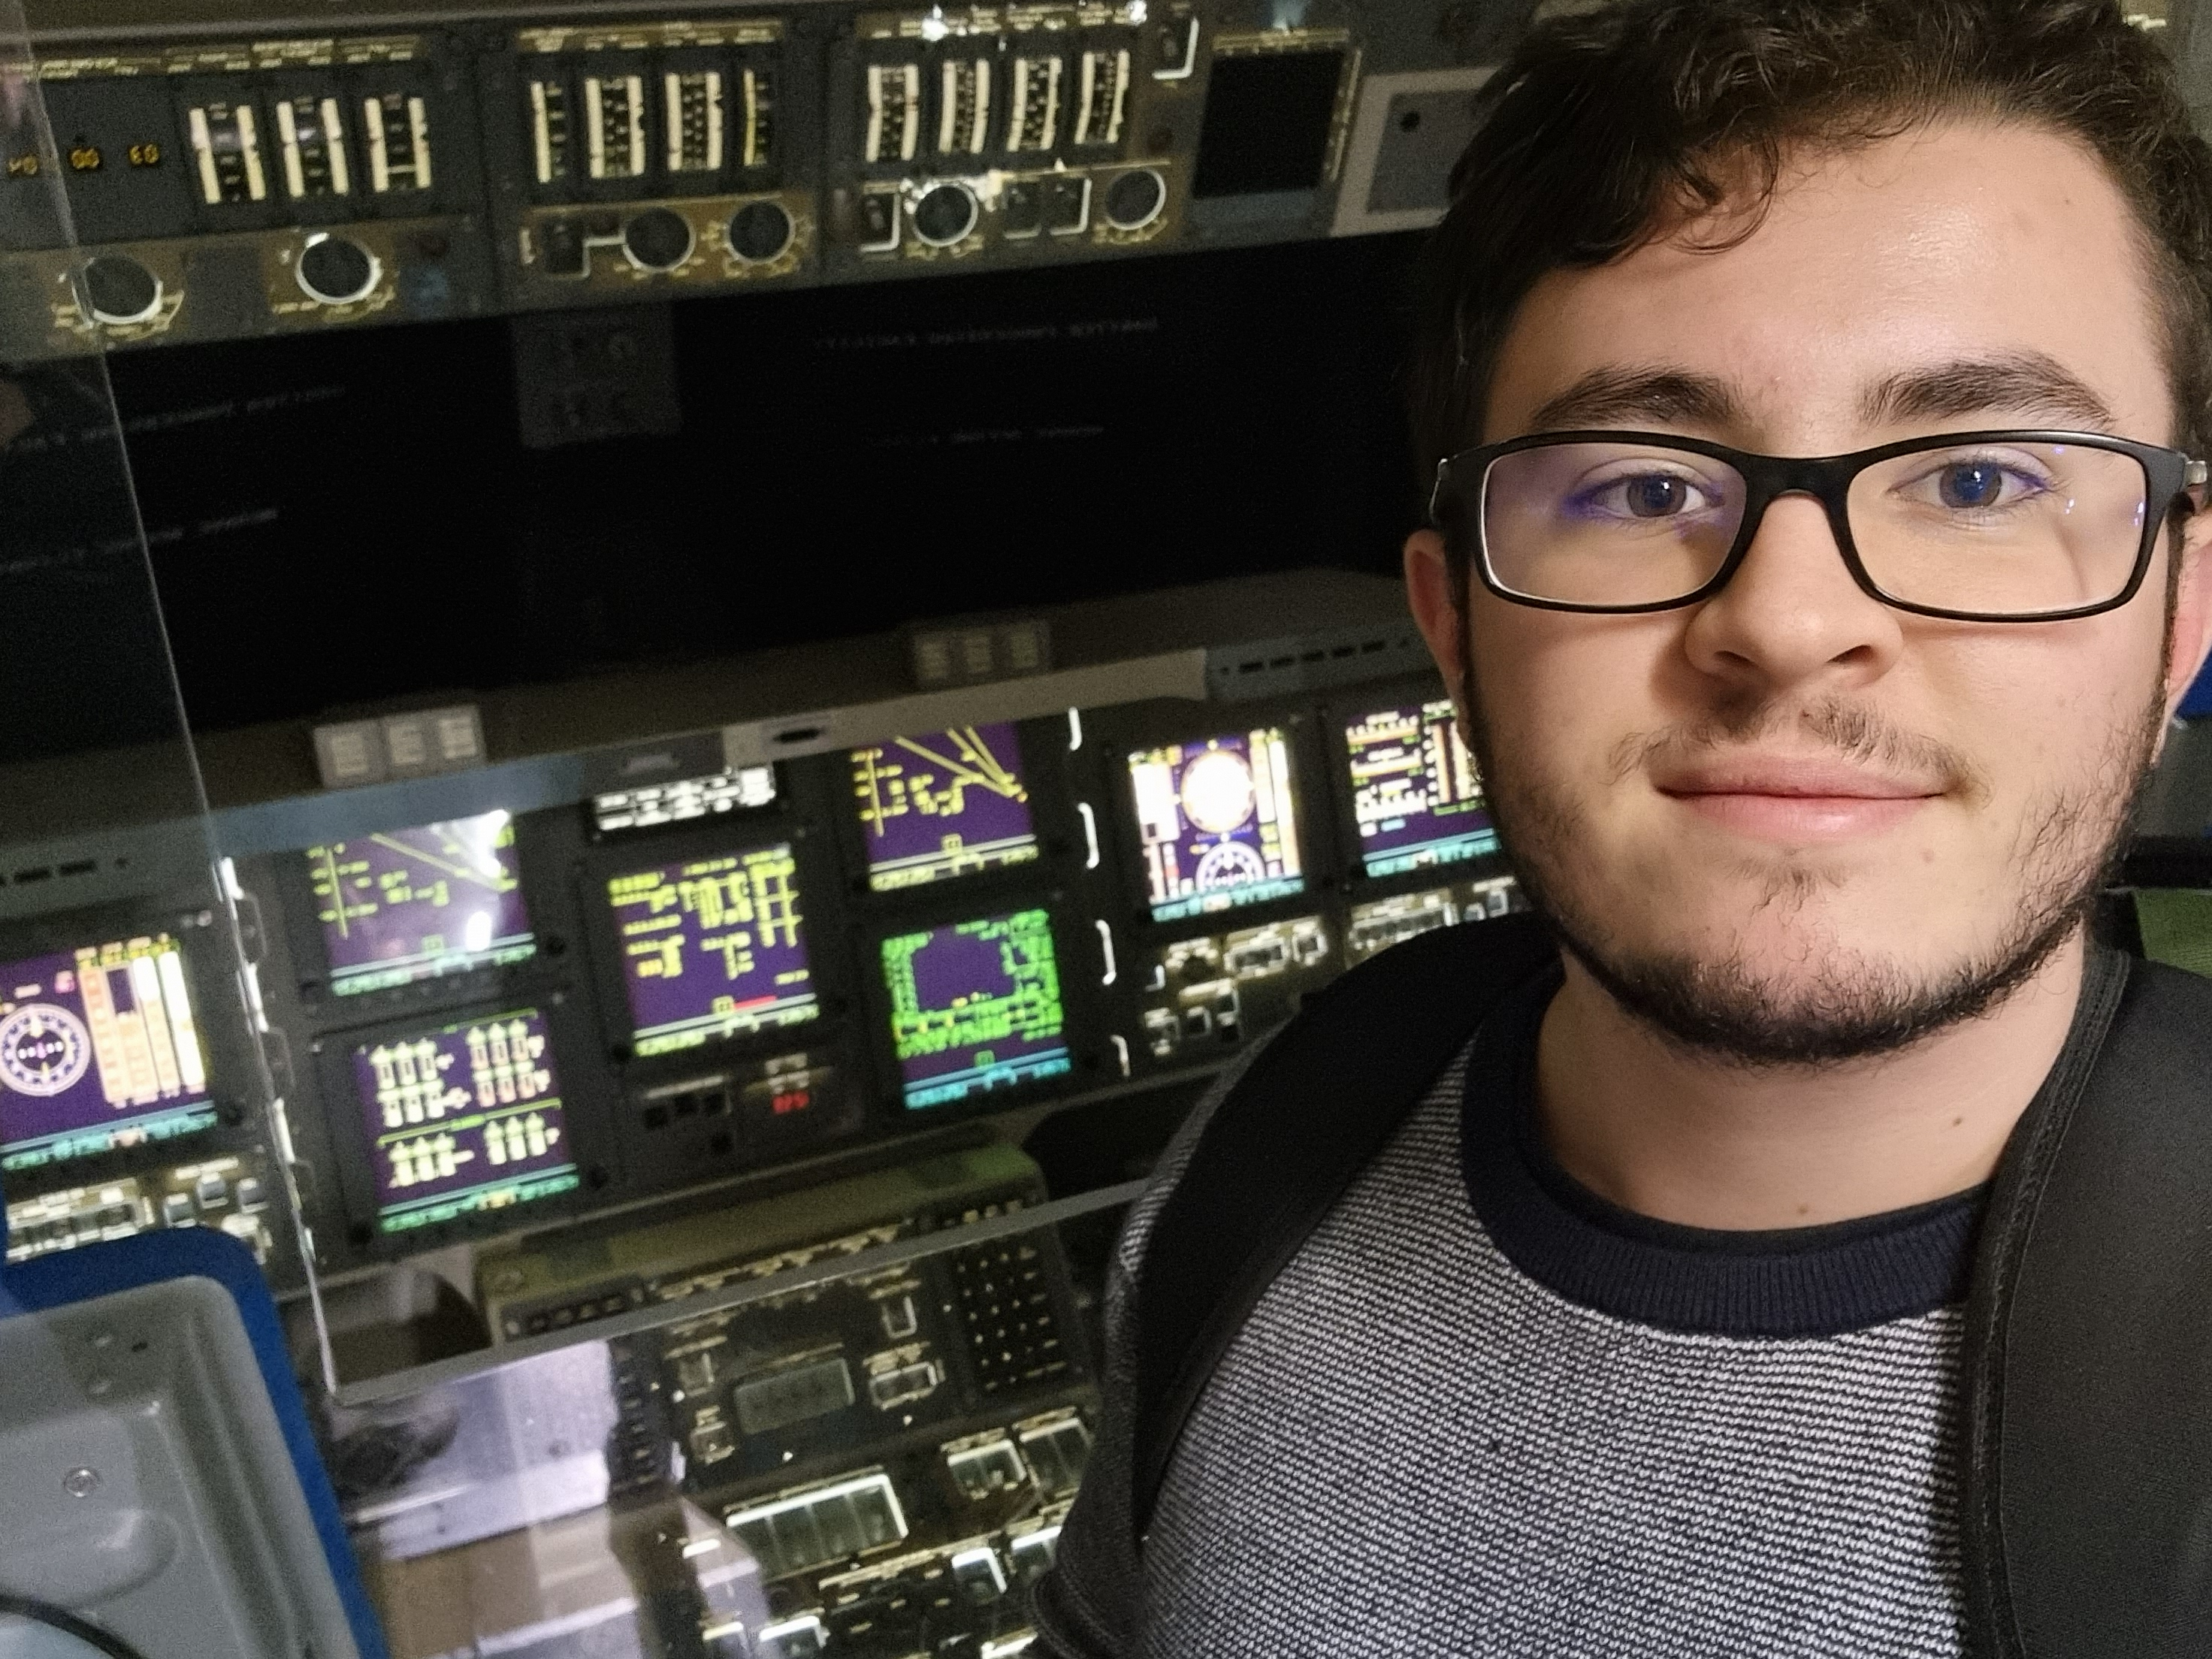
\includegraphics[width=\textwidth]{Jono_bio_pic.jpg}
\end{minipage}
\hspace{0.02\textwidth} % Space between image and text
\begin{minipage}{0.65\textwidth}
\textbf{Jonathan Faller} is an organiser of the Wits HPC Special Interest Group, and a previous winner of CHPC SCC 2022, and ISC SCC 2023 competitor for Team CHPC. He holds a degree in Biomedical Engineering (BEngSc) from the University of the Witwatersrand (enrolled in 2021), and is currently completing the 3rd year of study in Electrical Engineering - Information Engineering from the same institution. During his time with the Wits SIG, he has mentored teams to winning and coming second in the CHPC SCC 2023, and assisted Team CHPC of 2024 as the team captain from the previous year.
%they only have like 10 in person teams so I'm going to use Team CHPC to infer you've competed both in-person and online
\end{minipage}
\\\\\\
\noindent
\begin{minipage}{0.2\textwidth}
  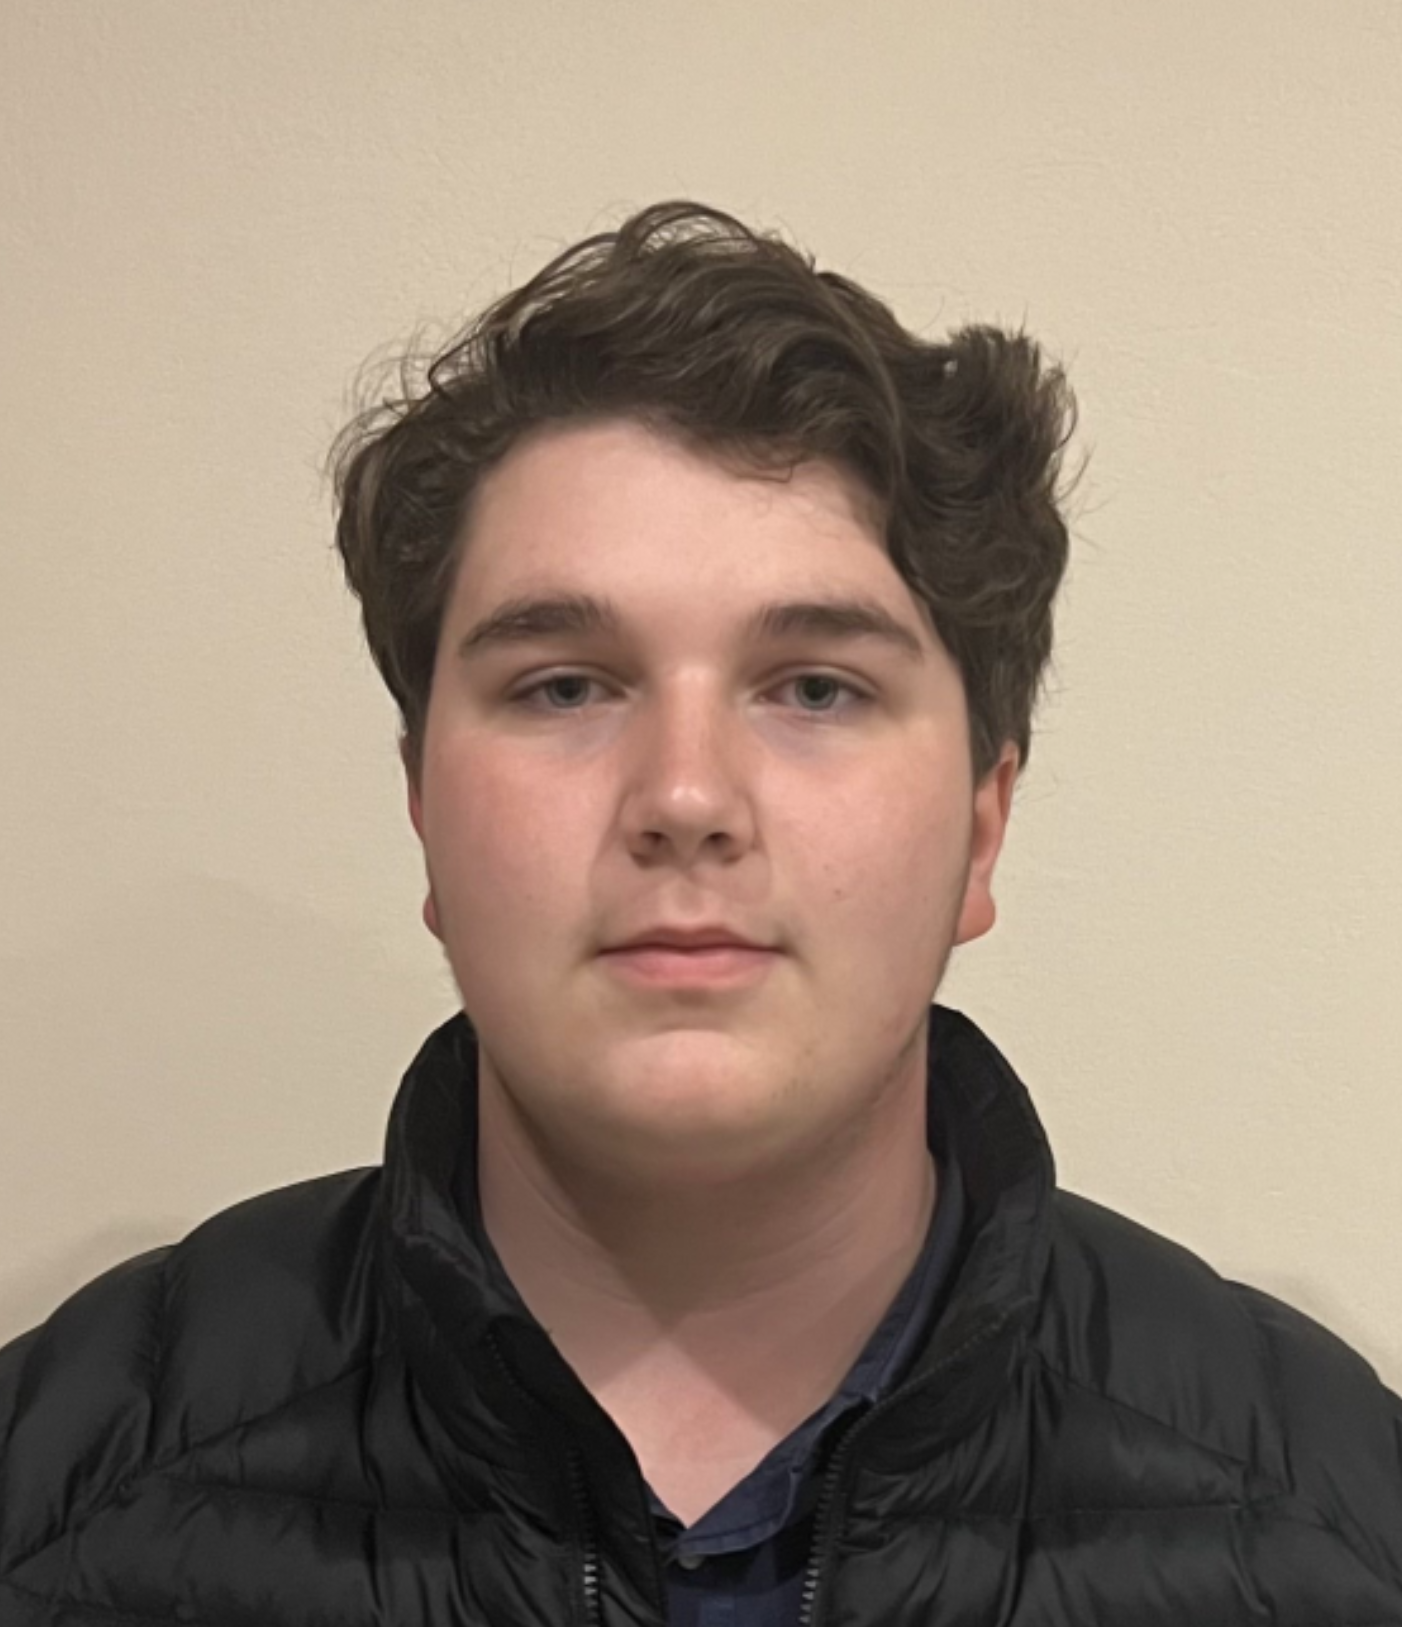
\includegraphics[width=\textwidth]{reinhard_bio.png}
\end{minipage}
\hspace{0.02\textwidth} % Space between image and text
\begin{minipage}{0.65\textwidth}
\textbf{Reinhard Jansen van Vuuren} is a final-year Biomedical Engineering student at the University of the Witwatersrand, Johannesburg (enrolled in 2022), with plans to continue into Electrical (Information) Engineering in 2025. He currently serves as an organiser for the Wits HPC Interest Group. He was the Team Captain of the winning team for the CHPC SCC 2023 and went on to represent Team CHPC at ISC SCC 2024. Reinhard is also mentoring teams for the CHPC SCC 2024. With a strong passion for high-performance computing, he is dedicated to advancing and developing the field of HPC.
%once again I'm using Team CHPC to infer South Africa
\end{minipage}
\\\\\\
\noindent
The remaining team members will be selected from the runner-up Wits teams that participate in this year's CHPC SCC. While the winning students will have the opportunity to join Team CHPC for an in-person experience at the ISC SCC, we aim to include the runner-ups in our team to ensure they also gain valuable experience. We will confirm their names within a week of the completion of the CHPC SCC 2024 on the 4th of December 2024. The names and photos of the selected students are provided below.
\\\\
\begin{minipage}{0.45\textwidth}
  \centering
  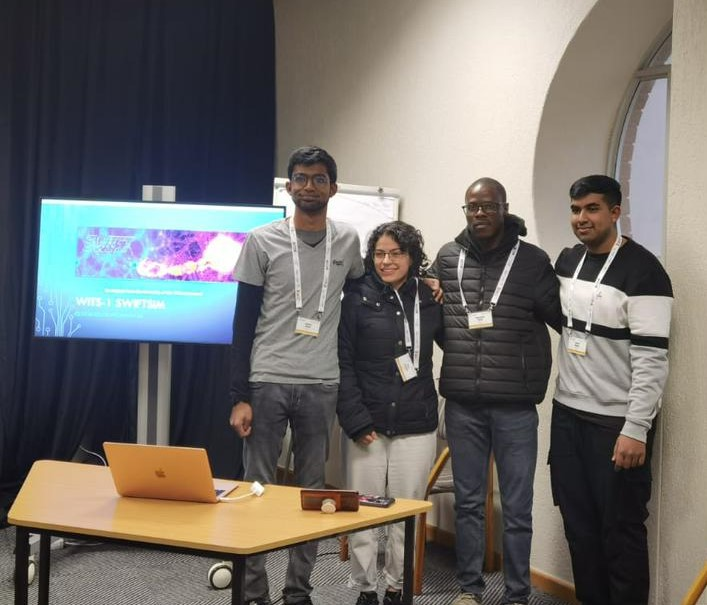
\includegraphics[width=0.7\textwidth]{wits1.jpg}
  \textbf{Rameez Mohammed Abdool, Clare Cordeiro, Mpumelelo Ntobi, Sachin Mohan} 
\end{minipage}
\hspace{0.05\textwidth} % Space between the images
\begin{minipage}{0.45\textwidth}
  \centering
  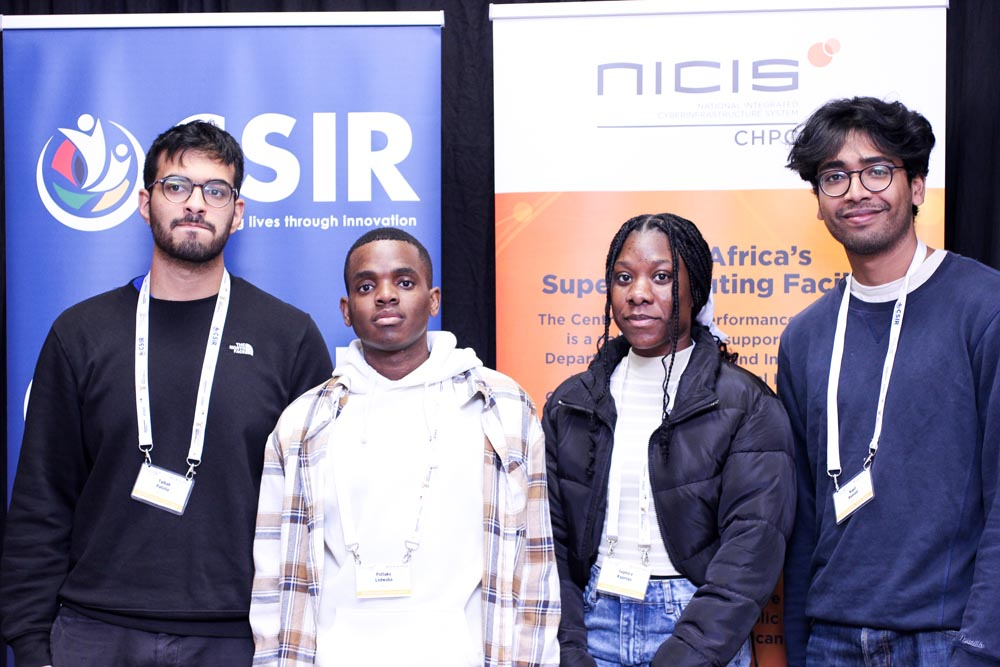
\includegraphics[width=0.9\textwidth]{witsa.jpg}
  \textbf{Talhah Patelia, Potlako Ledwaba, Mwanga Sefora Kapenga, Kapil Ramlall} 
\end{minipage}

\section{Why are we participating?}
\noindent
Our SIG supports students in progressing from beginner to intermediate levels in HPC within the Wits undergraduate community. We have consistently excelled at our local SCC and feel we have outgrown it. Our goal now is to extend our participation to the international level, beginning with the virtual ISC SCC 2025. By entering with an experienced team, we aim to establish a foundation that will enable us in future to include students new to SCCs as we grow more proficient. Ultimately, we aspire to compete in person at international events, strengthening our group's global presence and providing invaluable experience to our members.

\section{Why do we believe we have put together a winning team?}
\noindent
Our team is composed of experienced competitors who have actively participated in recent years, giving us a strong understanding of the current HPC landscape. Additionally, as facilitators of talks for undergraduate students, we are well-versed in the relevant topics. In the past, we've demonstrated our commitment by dedicating personal time to ISC SCC preparation, including conducting test benchmarks in advance, automating tasks through scripts, and holding regular weekly meetings to track progress. With our combined experience and reflections, we are eager to experiment with new approaches and strategies to achieve success.
\section{What sorts of diversity in skills do we possess?}
\noindent
Our team brings a diverse range of skills, with members from both Computer Science and Engineering backgrounds. Engineers excel at optimizing for hardware and system performance, while Computer Science students are skilled in debugging and software development. Additionally, some of our team members have experience as mentors, which has enhanced our leadership, communication, and problem-solving abilities. We also have expertise in scripting and automation, as well as experience with performance benchmarking and data analysis. This blend of technical and interpersonal skills allows us to approach problems from multiple angles and work effectively as a team
\section{Why will we work well together?} 
\noindent
Lily, Jonathan, and Reinhard currently serve as organisers for the Wits HPC SIG and mentors for the teams. We have collaborated closely over the past year, fostering a strong working relationship. The other team members are currently mentees and work directly with the Wits HPC SIG organisers, ensuring a seamless integration and effective teamwork. This established dynamic of mentorship and collaboration ensures we will work well together as a cohesive and experienced team.
\section{What experience do we have?}
\noindent
Jonathan Faller represented Team CHPC(virtually and in-person) for ISC SCC 2023, while Reinhard Jansen van Vuuren and Lily de Melo were part of Team CHPC(virtually and in-person) for ISC SCC 2024. The above students are also winners of the national CHPC SCC, which served as an essential stepping stone for international competition. Our team has garnered a wealth of experience having participated in three SCCs. 
\\\\
This background has equipped us with invaluable skills in building, configuring, and running high-performance applications. We have developed and optimized scripts and have experience working on both our clusters and production clusters. Our familiarity with these environments has refined our ability to handle performance tuning, resource management, and teamwork under intense, time-sensitive conditions. 
\section{How will we work together to tune and optimise the application set?}
\noindent
We will divide the team into smaller groups to work collaboratively on different applications. Each group will research the applications and test various configurations, including different compilers, MPIs, and dependencies. To streamline the process, we will use scripts to automate testing and simplify configuration management. Regular weekly meetings will be held to discuss progress, share feedback, and ensure that we stay on schedule.
\section{The commitment of the institution to educating the broader student community about the usefulness and accessibility of High Performance Computing at your institution}
\noindent
The Wits HPC SIG plays a key role in educating the broader university community about the value of High Performance Computing. We aim to set up a SIG cluster that will provide a practical aspect to our talks and give SIG members direct access to HPC resources. The university has shown strong support in this endeavour and is one of our projects for 2025. We believe that excelling in this competition will not only further raise awareness but also help us expand our reach, motivating industry partners to collaborate with us and support our initiatives.
\section{Explain how HPC is integrated in the educational curriculum of the proposing institution}
\noindent
Our group plays a central role in introducing undergraduates to HPC, providing hands-on experience and practical knowledge. Our group's curriculum has been uploaded to a \href{https://github.com/WitsHPC/HPC-InterestGroup}{GitHub Repository}. Additionally, the university offers an Honours-level course in Computer Science titled \textit{High Performance Computing and Scientific Data Management}, as well as a fourth-year engineering course called \textit{Data Intensive Computing in Data Science}. Both of which teach concepts of parallel computing and other relevant subject matter.
\section{Do we have a HPC cluster at our educational institution to practice the benchmarks}
\noindent
Currently, we have access to decommissioned hardware, which we have repurposed for our HPC needs as we work toward setting up a dedicated SIG cluster. In the meantime, this allows us to practice and test benchmarks effectively. Additionally, the university’s School of Computer Science operate their own clusters, which we can access if needed.
\\\\
We are also currently reaching out to industry partners for sponsorship of a small competition-type cluster for practice and learning for SCC teams.
\section{Do we wish to participate in the in-person only, virtual only, or both?}
\noindent
We are participating only in the virtual competition this year, but our goal is to compete in person in future years.
%\bibliographystyle{ieeetr}
%\bibliography{references}
\label{lastBodyPage}
%\end{multicols*}
\newpage
\fancyfoot[C]{Page \thepage\ of \pageref{lastRomanPage}}
\pagenumbering{roman}  
\appendices
\label{lastRomanPage}

\end{document}

